\subsection*{\textbf{Задание 12.4} Построение 3D-графиков, заданных параметрически.}
\begin{itemize}
    \item Постройте график, изображающий лист Мёбиуса.
    Формулы для его задания:
    \[
        \begin{cases}
            X(u,t) = (r+h\cdot u \cdot \cos(n\cdot t/2))\cdot \cos t \\
            Y(u,t) = (r+h\cdot u \cdot \cos(n\cdot t/2))\cdot \sin t \\
            Z(u,t) = h \cdot u \cdot \sin(n \cdot t/2) \\
        \end{cases}
    \]
    \textbf{n} -- количество скручиваний; \\
    \textbf{r} -- радиус; \\
    \textbf{h} -- ширина; \\
    Рассмотрите интервалы $t$ от $0$ до $2\pi, u$ от $0$ до $3$.
    \item Постройте поверхность $f(x,y) = 2\cos(x) + y$, где $x$ и $y$, изменяются от $-\pi$ до $\pi$.
\end{itemize}
Результаты выполнения задания сохраните и продемонтрируйте преподавателю.

\begin{figure}[H]
    \renewcommand{\figurename}{Рисунок}
    \centering{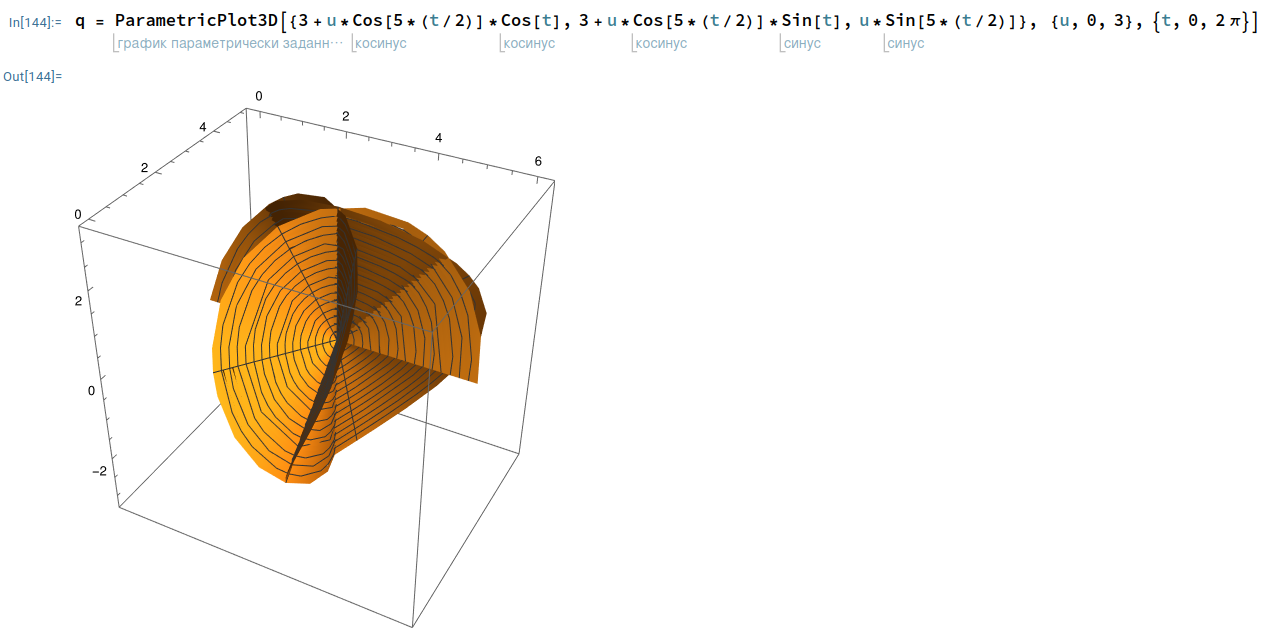
\includegraphics[scale=0.40]{body/img/12_4_1.png}}
    \label{fig:image_12_4_1}
\end{figure}

\begin{figure}[H]
    \renewcommand{\figurename}{Рисунок}
    \centering{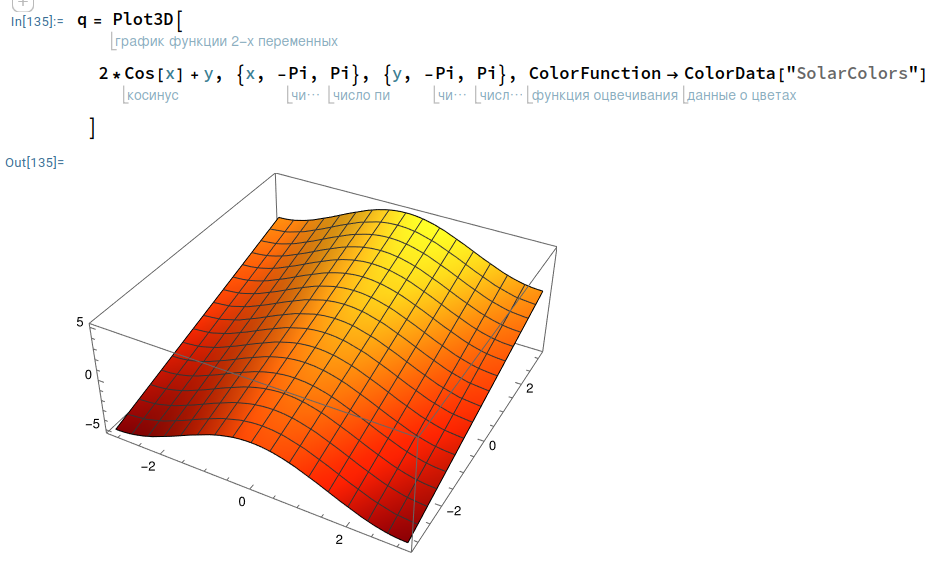
\includegraphics[scale=0.50]{body/img/12_4_2.png}}
    \label{fig:image_12_4_2}
\end{figure}